\chapter{Appendix: Implementation and Experiments Artifacts}

This chapter includes references to the implementation Data Persistence
Implementation covering its design and architecture. Also, some of the
implementation details of the DSP Data Persistence component designed in
Chapter 6 are presented, showing the generated experiment artifacts. While
this section does not include all the related source-codes, the remainder can
be downloaded directly from the Subversion repository branch at
http://code.google.com/p/netbeams/source/browse/\#svn/branches/marcello/persistence/.

\section{DSP Platform Deployment Details}
\label{sec:dsp-data-persistence-implementation}

The DSP Data Persistence component was implemented using the Java Programming
language, on top of the OSGi Framework. This section describes the setup
process of the implementation, as well as the artifacts use during the
implementation, which will be listed in the appendix section.

The structure of the artifacts implemented for the DSP Data Persistence
Component follow the conventions of the NetBEAMS implementation
\cite{netbeams-dsp-architecture}, where the main directory
\textbf{PERSISTENCE-DIR}, depicted by Figure
\ref{fig:dsp-data-persistence-dir-checkedout}, holds each of the development
artifacts.

\begin{itemize}
  \item \textbf{DSPDataPersistence}: Main directory with the build.xml (Listing
  \ref{file:dsp-build.xml}) and other Eclipse-related artifacts. The other
  major directories are also listed;
  \item \textbf{META-INF}: this directory contains the descriptor file for
  the OSGi Framework, in this case, the MANIFEST.MF;
  \item \textbf{src}: the main directory structure for the source-code
  implemented. Note that it follows the Java specification for packaging, and
  therefore, lists the package org.netbeams.dsp.persistence as the main
  package, including the layers controller, model and OSGi.
\end{itemize}

\begin{figure}[!h]
  \centering
  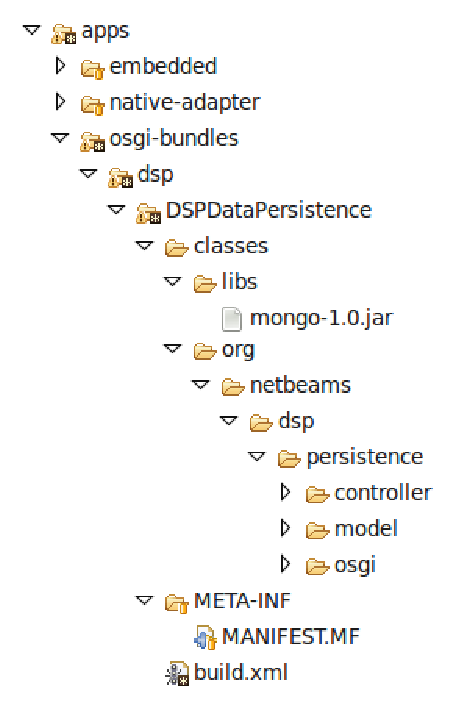
\includegraphics[scale=0.65]{../diagrams/dsp-data-persistence-dir-checkedout}
  \caption{The DSP Data Persistence Directory Structure}
  \label{fig:dsp-data-persistence-dir-checkedout}
\end{figure}

\subsection{OSGi Deployment Process}
\label{sec:dsp-component-osgi-deployment}

Since each NetBEAMS component is managed by an OSGi component and its
infrastructure, this section describes the basic functionality of the
OSGi platform \cite{osgi}, a framework was conceived to support
modularity in terms resources-limited environments such mobile devices and
vehicles, but it was first widely deployed on Eclipse IDE\footnote{Integrated
Development Environment}. It promotes reusable loosely-coupled modules to be
integrated using the Java Programming Language \cite{java}. The most basic
layers of the OSGi Framework depicted in Figure \ref{fig:layering-osgi} are as
follows:

\begin{itemize}
  \item \textbf{Module Layer}: manages the OSGi bundles deployed on the
  OSGi Platform, providing the necessary "wiring" of the components. In other words,
  the modules, called OSGi Bundles, can export and/or import packages in the
  level of a Java Class managed by the OSGi Framework;
  \item \textbf{Service Layer}: responsible for the interoperability between two
  or more bundles, enabling the bundles to register services offered by
  the its specification;
  \item \textbf{Execution Layer}: executes the bundles, managing and changing
  their lifecycle through the bundle execution.
\end{itemize}

\begin{figure}[!h]
  \centering
  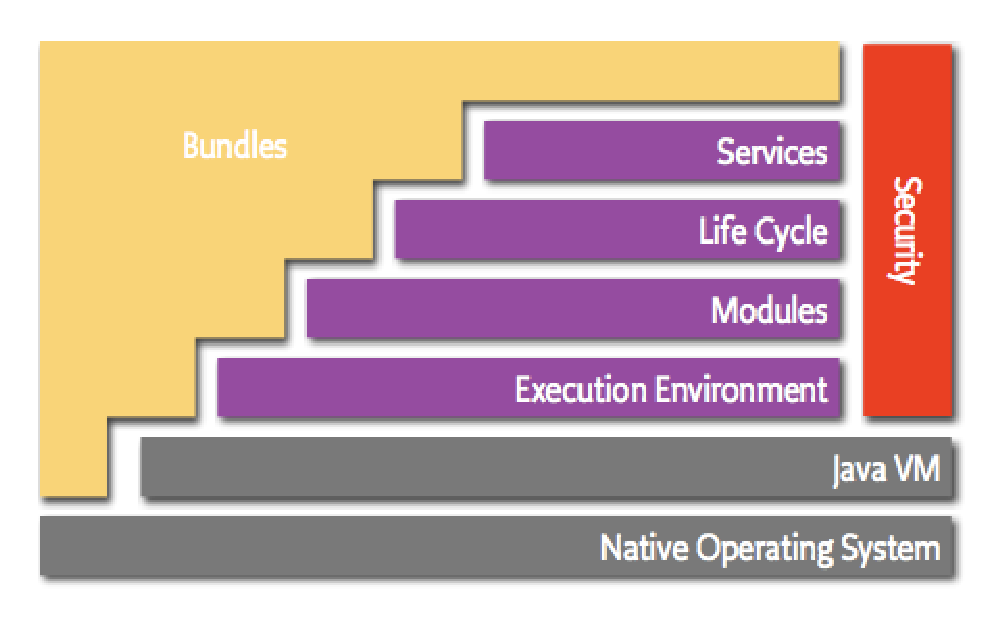
\includegraphics[scale=0.65]{../diagrams/layering-osgi}
  \caption{The OSGi Framework Layers}
  \label{fig:layering-osgi}
\end{figure}

NetBEAMS uses the concept of the modularization through the use of the
Producer-Consumer paradigm described in the previous section. Since the DSP
Components are essentially OSGi bundles, the interoperability between
them is given by the OSGi Framework, described by an artifact called
MANIFEST.MF (Listing \ref{file:OSGi-manifest}). In general, an OSGi bundle must
provide specifications that describe the module to be published into the OSGi
Framework. In this way, the main properties of the OSGi MANIFEST.MF artifact
can used by the DSP Data Persistence can be summarized as follows:

\begin{itemize}
  \item \textbf{Bundle-Activator}: The name of the instance of an OSGi
  Activator class, responsible to manage the bundle. The implemented class
  ``DataPersistenceActivator'' provides the activation mechanisms for the
  services of the DSP Data Persistence Component;
  \item \textbf{Bundle-ClassPath}: the necessary Java Jars list needed to run
  the bundle. It lists the mongoDB Java driver as one of the required
  dependencies deployed in the same package;
  \item \textbf{Import-Package}: the Java Packages needed by the DSP Data
  Persistence Component Bundle. These Java Packages must be provided by other
  DSP components, forcing the execution to be dependent on those packages.
  They are provided through a section called ``Export-Package'', in other
  OSGi bundles and as it is shown in Listing \ref{file:OSGi-manifest}, they
  are can be from different packages.
\end{itemize}

Once the OSGi bundle is installed into the OSGi Platform, it will be managed by
the OSGi Execution layer and change the bundle state according to its
lifecycle. Therefore, the packaging of the OSGi source-code is done using a
JAR\footnote{Java Archival Repository} artifact specification
\cite{java-tutorial}. The DSP Platform is bundled into a JAR created by the
Apache ANT build script \cite{apache-ant}, as shown in Listing
\ref{file:dsp-build.xml}. The task ``dsp-data-persistence.all'' compiles all
the source-code created from the design of Chapter 6 and packages
everything into an artifact name ``DSPDataPersistence-x.x.jar'', where x.x is
the version of the bundle. Figure \ref{fig:dsp-runtime-dir} shows the DSP Data
Persistence file under the directory ``\textbf{RUNTIME-DIR}/deployment/''.

\begin{figure}[!h]
  \centering
  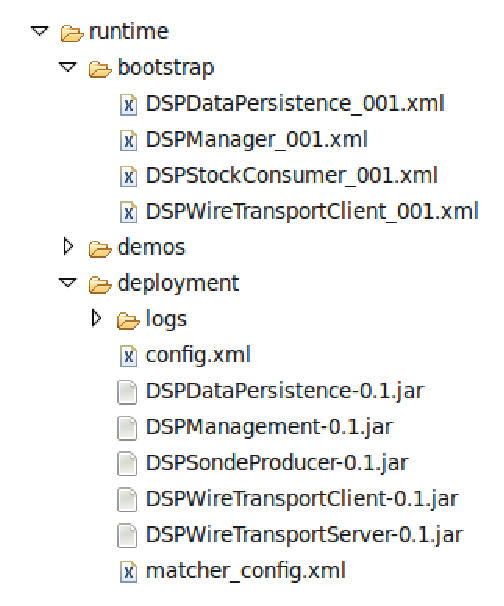
\includegraphics[scale=0.65]{../diagrams/dsp-runtime-dir}
  \caption{The DSP Runtime Dir}
  \label{fig:dsp-runtime-dir}
\end{figure}

\subsection{DSP Data Persistence into the DSP Platform}
\label{sec:dsp-persistence-boostrap}

When the new component was developed and deployed by editing two main
configuration descriptors:

\begin{itemize}
  \item \textbf{config.xml}: the DSP Data Persistence is added to the DSP
  Platform by adding an entry for the component's OSGi Bundle artifact. This
  artifact can be seen in Listing \ref{file:dsp-config.xml};
  \item \textbf{matcher\underline{ }config.xml}: the addition of the rules that
  filters DSP Messages to the DSP Data Persistence component;
  \item \textbf{DSPDataPersistence\underline{ }001.xml}: depicts the bootstrap
  message for the DSP Data Persistence Component, as shown in Listing 
  \ref{file:dsp-data-persistence-bootstrap.xml}.
\end{itemize}

The first configuration artifact enables NetBEAMS to initialize the
descriptor of the component, as shown in Listing \ref{file:dsp-config.xml}.
The component is added with the highest priority, since it contains
dependencies to other DSP Components.

\section{mongoDB Deployment Details}
\label{sec:mongodb-deployment}

MongoDB was the selected technology described in Chapter 5 because of its
features. It provides data persistence based on collections of data, stored
using BSON \cite{bson}, a binary representation the JSON data representation
format. mongoDB uses the abstraction of programming language to represent the
basic CRUD operators, as well as the regular functionalities provided by any
type of database system such as indexing and users management. As it's stated
in their web site, mongoDB "bridges the gap between key/value stores, which
are fast and highly scalable, traditional RDBMS systems (deep in
functionality)".

\begin{itemize}
  \item mongoDB implements a document-oriented structure, which is similar to
  Key-Value Pairs;
  \item mongoDB is written in C++, and therefore, can is available in any major
  platform, as well as offers a broad range of API drivers written in
  different languages such as Java, Python, Perl and Ruby;
  \item mongoDB has support to distributed systems such as Master-Slave
  Replication, and horizontal database partitioning, referred to as Database
  Shards.
\end{itemize}

The artifacts of the mongoDB are located in the ``thirdparty'' directory of the
NetBEAMS resources directory. The build script from the DSP Data Persistence
component can be executed to produce the persistence directory structure for
NetBEAMS, as described in Figure \ref{fig:dsp-persistence-system-dir}.

\begin{figure}[!h]
  \centering
  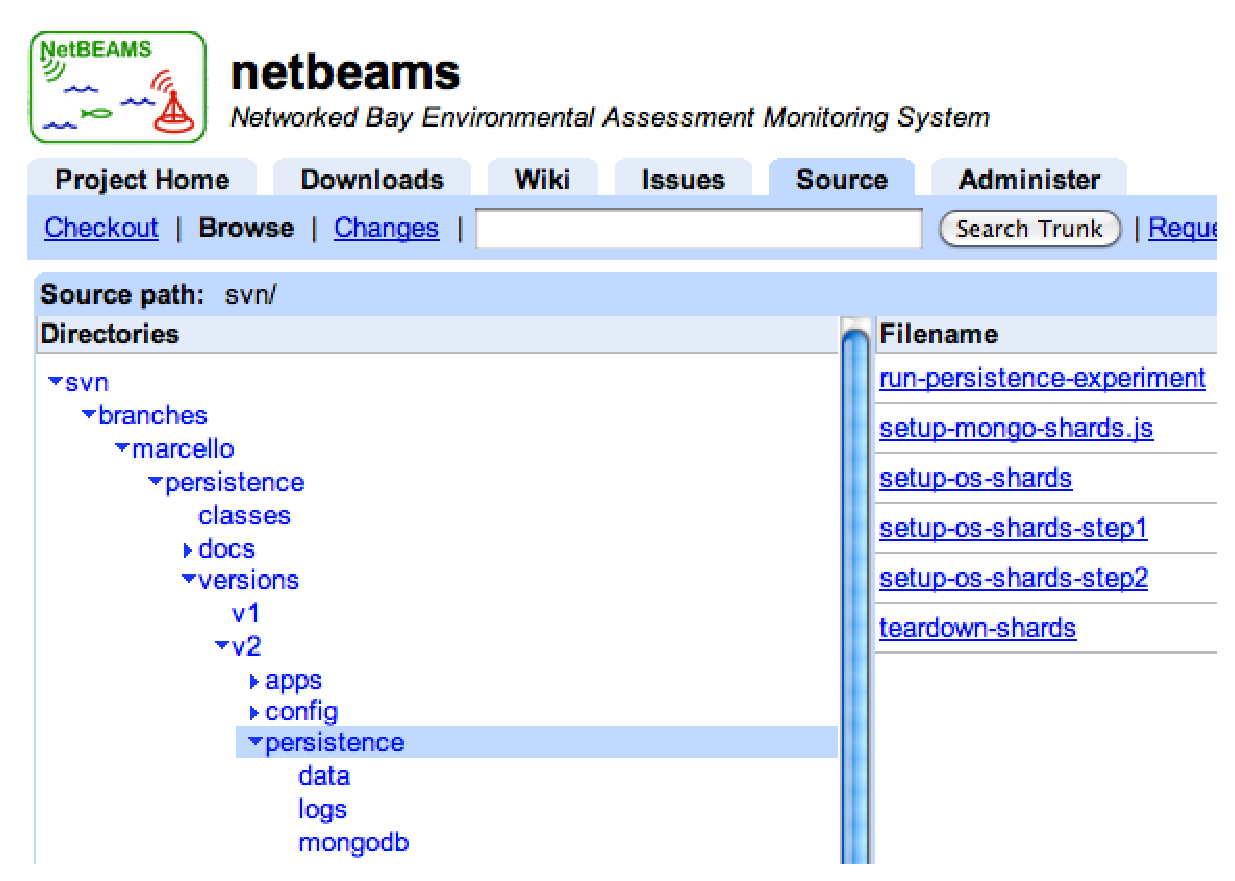
\includegraphics[scale=0.65]{../diagrams/dsp-persistence-system-dir}
  \caption{DSP Data Persistence directory}
  \label{fig:dsp-persistence-system-dir}
\end{figure}

\subsection{Using the Client and Server}

In order to start the server, the command-line shown in Listing
\ref{cmd:mongodb-server-start} is used, where the data is configured to be
stored at the directory  ``./data/'', relative to the directory shown in the
shell. Also, the port number where the server listens to the client
connections is give as port ``20000". Once the server is running, any client
application can access to the server. For example, in order to connect the DSP
Data Persistence component, the port 20000 is an optional value be provided in
the DSP Data Persistence bootstrap message, as shown in Listing
\ref{file:dsp-data-persistence-bootstrap.xml}. Although mongoDB offers the
option to run with its specific default port number, it is recommended to
assign different ports, once the use of shards requires different port numbers
for each of the shard servers. An example of accessing mongoDB using a shell
client is shown in Listing \ref{cmd:mongodb-client-start}.

\lstset{label=cmd:mongodb-server-start,caption=Starting the Server}
\begin{lstlisting}
marcello-de-saless-macbook-pro:persistence marcello$ mongod --dbpath data/ --port 20000 &

Wed Dec  9 01:39:51 Mongo DB : starting : pid = 10096 port = 20000 dbpath = data/ master = 0 slave = 0  64-bit 
Wed Dec  9 01:39:51 db version v1.1.4, pdfile version 4.5
Wed Dec  9 01:39:51 git version: ad7fc8908396a3351a0f07bb1e2fc4baba2802ad
Wed Dec  9 01:39:51 sys info: Darwin erh2.10gen.cc 9.6.0 Darwin Kernel Version 9.6.0: Mon Nov 24 17:37:00 PST 2008; root:xnu-1228.9.59~1/RELEASE_I386 i386 BOOST_LIB_VERSION=1_37
Wed Dec  9 01:39:51 waiting for connections on port 20000
\end{lstlisting}

\lstset{label=cmd:mongodb-client-start,caption=Starting the Server}
\begin{lstlisting}
marcello@netbeams-dev:~/workspaces $ mongo 192.168.1.2:20000/netbeams
MongoDB shell version: 1.1.4
url: 192.168.1.2:20000/netbeams
connecting to: 192.168.1.2:20000/netbeams
type "help" for help
\end{lstlisting}

\section{Experiments Execution}
\label{sec:experiment-execution}

The experiments conducted using mongoDB can be summarized by the different data
access methods provided by the technology. Each subsection describes these 
methods. The server could be started using the commands specified in the
previous section.

\lstset{label=cmd:run-persistence-experiment,caption=Running main experiment
shell script}
\begin{lstlisting}
marcello@netbeams-dev:~/workspaces/netbeams/versions/v2/persistence$ ./run-persistence-experiment 
#######  NetBEAMS Experiments - Persistence on MongoDB  ########

Usage: ./run-persistence-experiment X, where X is the size of the workload to be inserted from NetBEAMS YSI Data Handler to mongoDB
\end{lstlisting}


\subsection{Data Access Using Database Shell}
\label{sec:mongodb-user-experience}

The iterative mongo client shell offers users to verify and navigate on a
given database and its collections. This first section shows the connection of
the mongo client to the database ``netbeams'' as on Listing
\ref{cmd:mongodb-server-start}. The execution of the operation to count the
existing number of documents in the mongoDB collection ``netbeams'' is shown in
Listing \ref{cmd:mongodb-count}. It highlights the query for the collections
available \cite{mongodb} in the netbeams database.

\lstset{label=cmd:mongodb-count,caption=Starting the Server}
\begin{lstlisting}
...
...
connecting to: 192.168.1.2:20000/netbeams
type "help" for help
> show collections
SondeDataContainer
system.indexes
> db.SondeDataContainer.count()
2419200
\end{lstlisting}

An example about data retrieving of a random document from the collection
``netbeams'', ``findOne()'' is documented to provide this support as shown in
Listing \ref{cmd:mongo-findone}. The output is the actual instance of a
document, showing all the collected data in the key ``observation'', and the
provenance metadata in the keys ``sensor.location'' and ``sensor.time''.

\lstset{label=cmd:mongo-findone,caption=Querying the database: one item}
\begin{lstlisting}
> db.SondeDataContainer.findOne()
{
    "_id" : ObjectId("5d6f40078ec8074bba980900"),
    "message_id" : "020d82e1-18b2-4fe2-800c-a0f68e22ea86",
    "sensor" : {
        "ip_address" : "192.168.0.91",
        "location" : {
            "latitude" : 37.89155,
            "longitude" : -122.4464
        }
    },
    "time" : {
        "valid" : "Wed Nov 04 2009 02:30:12 GMT-0800 (PST)",
        "transaction" : "Sat Nov 21 2009 03:01:33 GMT-0800 (PST)"
    },
    "observation" : {
        "WaterTemperature" : 88.58,
        "SpecificConductivity" : 180.5,
        "Conductivity" : 167.3,
        "Resistivity" : 491.89,
        "Salinity" : 0.06,
        "Pressure" : 1.109,
        "Depth" : 2.642,
        "pH" : 7.11,
        "pHmV" : -42.9,
        "Turbidity" : 0.2,
        "ODOSaturation" : 72.4,
        "ODO" : 10.85,
        "Battery" : 2.7
    }
}
\end{lstlisting}

The query based on attributes can be done using the "dot" notation, as the user
can navigate through the JSON documents. Additionally, the use of internal
functions is provided by mongoDB on the result of others. The example in
Listing \ref{cmd:mongo-find-list} counts the number of documents with the key
"data.ph" equals to "5.64".

\lstset{label=cmd:mongo-find-list,caption=Execution of mongo client}
\begin{lstlisting}
> db.SondeDataContainer.find({"data.ph":5.64)}).count()
1226
\end{lstlisting}

The following example is the output of the first 2 documents from the same
previous query using the function ``limit()``, as shown in Figure
\ref{cmd:mongo-find-limit}. The function ``limit()'' is used to decrease the
number of items returns by the given number.

\lstset{label=cmd:mongo-find-limit,caption=Query Element with specific
projection limiting the result set size}
\begin{lstlisting}
> db.SondeDataContainer.find({"data.ph":5.64}).limit(2)
{"_id" :  ObjectId( "d36f4007b7e7ac4a03c60000")  , "sensor_ip_address" : "192.168.0.136" , "message_id" : "7b6624d6-0ca1-4cba-a343-f166e88da73b"
, "transaction_time" : 1252845473412 , "fact_time" : 1252845346000 , "data" : {"temperature" : "45.01" , "sp_condition" : "37.6" ,
"condition" : "145.8" , "resistence" : "159.77" , "salinitude" : "0.0" , "pressure" : "0.391" , "depth" : "0.46" , "ph" : "5.64" ,
"pH_mv" : "-62.1" , "odo_sat" : "89.7" , "odo_condition" : "59.34" , "turbidity" : "0.0" , "battery" : "9.4"}}
{"_id" :  ObjectId( "d36f4007b7e7ac4a1fc80000")  , "sensor_ip_address" : "192.168.0.136" , "message_id" : "7b6624d6-0ca1-4cba-a343-f166e88da73b" ,
"transaction_time" : 1252845473412 , "fact_time" : 1252845346000 , "data" : {"temperature" : "46.71" , "sp_condition" : "60.8" ,
"condition" : "160.6" , "resistence" : "1399.4" , "salinitude" : "0.01" , "pressure" : "1.057" , "depth" : "2.485" , "ph" : "5.64" ,
"pH_mv" : "-16.3" , "odo_sat" : "58.8" , "odo_condition" : "19.29" , "turbidity" : "0.2" , "battery" : "9.2"}}
>
\end{lstlisting}

\subsection{Data Access Using APIs}
\label{sec:dsp-mongodb-rest-ws}

The mongoDB server offers different drivers to access the data, as well as the
REST Web Services. In order to get the results using the REST Web Services
interdace, the request can be issued using a web browser. For instance, the
request to the documents using the HTTP Request Variables to filter by the
fields as shown in Listing \ref{cmd:mongo-rest-request}.

\lstset{label=cmd:mongo-rest-request,caption=REST HTTP Interface Example}
\begin{lstlisting}
http://192.168.1.2:28017/netbeams/SondeDataContainer/?limit=-3&filter_observation.Conductivity=104.5

HTTP/1.0 200 OK
x-action:
x-ns: netbeams.SondeDataContainer
Content-Type: text/plain;charset=utf-8

{
  "offset" : 0,
  "rows": [
    { "_id" : { "$oid" : "616f400784ba194bc2dee200" }, 
      "message_id" : "c76a9898-1eee-4463-bf5d-d40a7a8af6e3", 
      "sensor" : { "ip_address" : "192.168.0.60", 
                   "location" : {
                       "latitude" : 37.89155, "longitude" : -122.4464} 
                 }, 
      "time" : { 
               "valid" : { "$date" : 1261229067000 },
               "transaction" : { "$date" : 1259977271704 } 
               },
      "observation" : { 
                "WaterTemperature" : 51.29, "SpecificConductivity" :110.7,
                "Conductivity" : 104.5, "Resistivity" : 1710.07, "Salinity" :0.01, 
                "Pressure" : 1.094, "Depth" : 1.808, "pH" : 3.04,
                "pHmV" : -46.4, "Turbidity" : 0.2, "ODOSaturation" :59, 
                "ODO" : 10.66, "Battery" : 7.1 
                } 
                ......
                ...... More records....
   } 
   "total_rows" : 3 , "query" : {} , "millis" : 91 }
\end{lstlisting}

\subsection{Visualizing Data on the Browser}

Data visualisation tools for mongoDB is slowly being developed by open-source
developers. Futon4mongodb, one of the open-source tools developed to visualise
mongoDB data, is an adaptation of another software developed for CouchDB
\cite{couchdb}. Figure \ref{fig:view-collections-instance-browser-futondb}
shows one single collection for the YSI data containing of 1 million objects.

\begin{figure}[h]
  \centering
  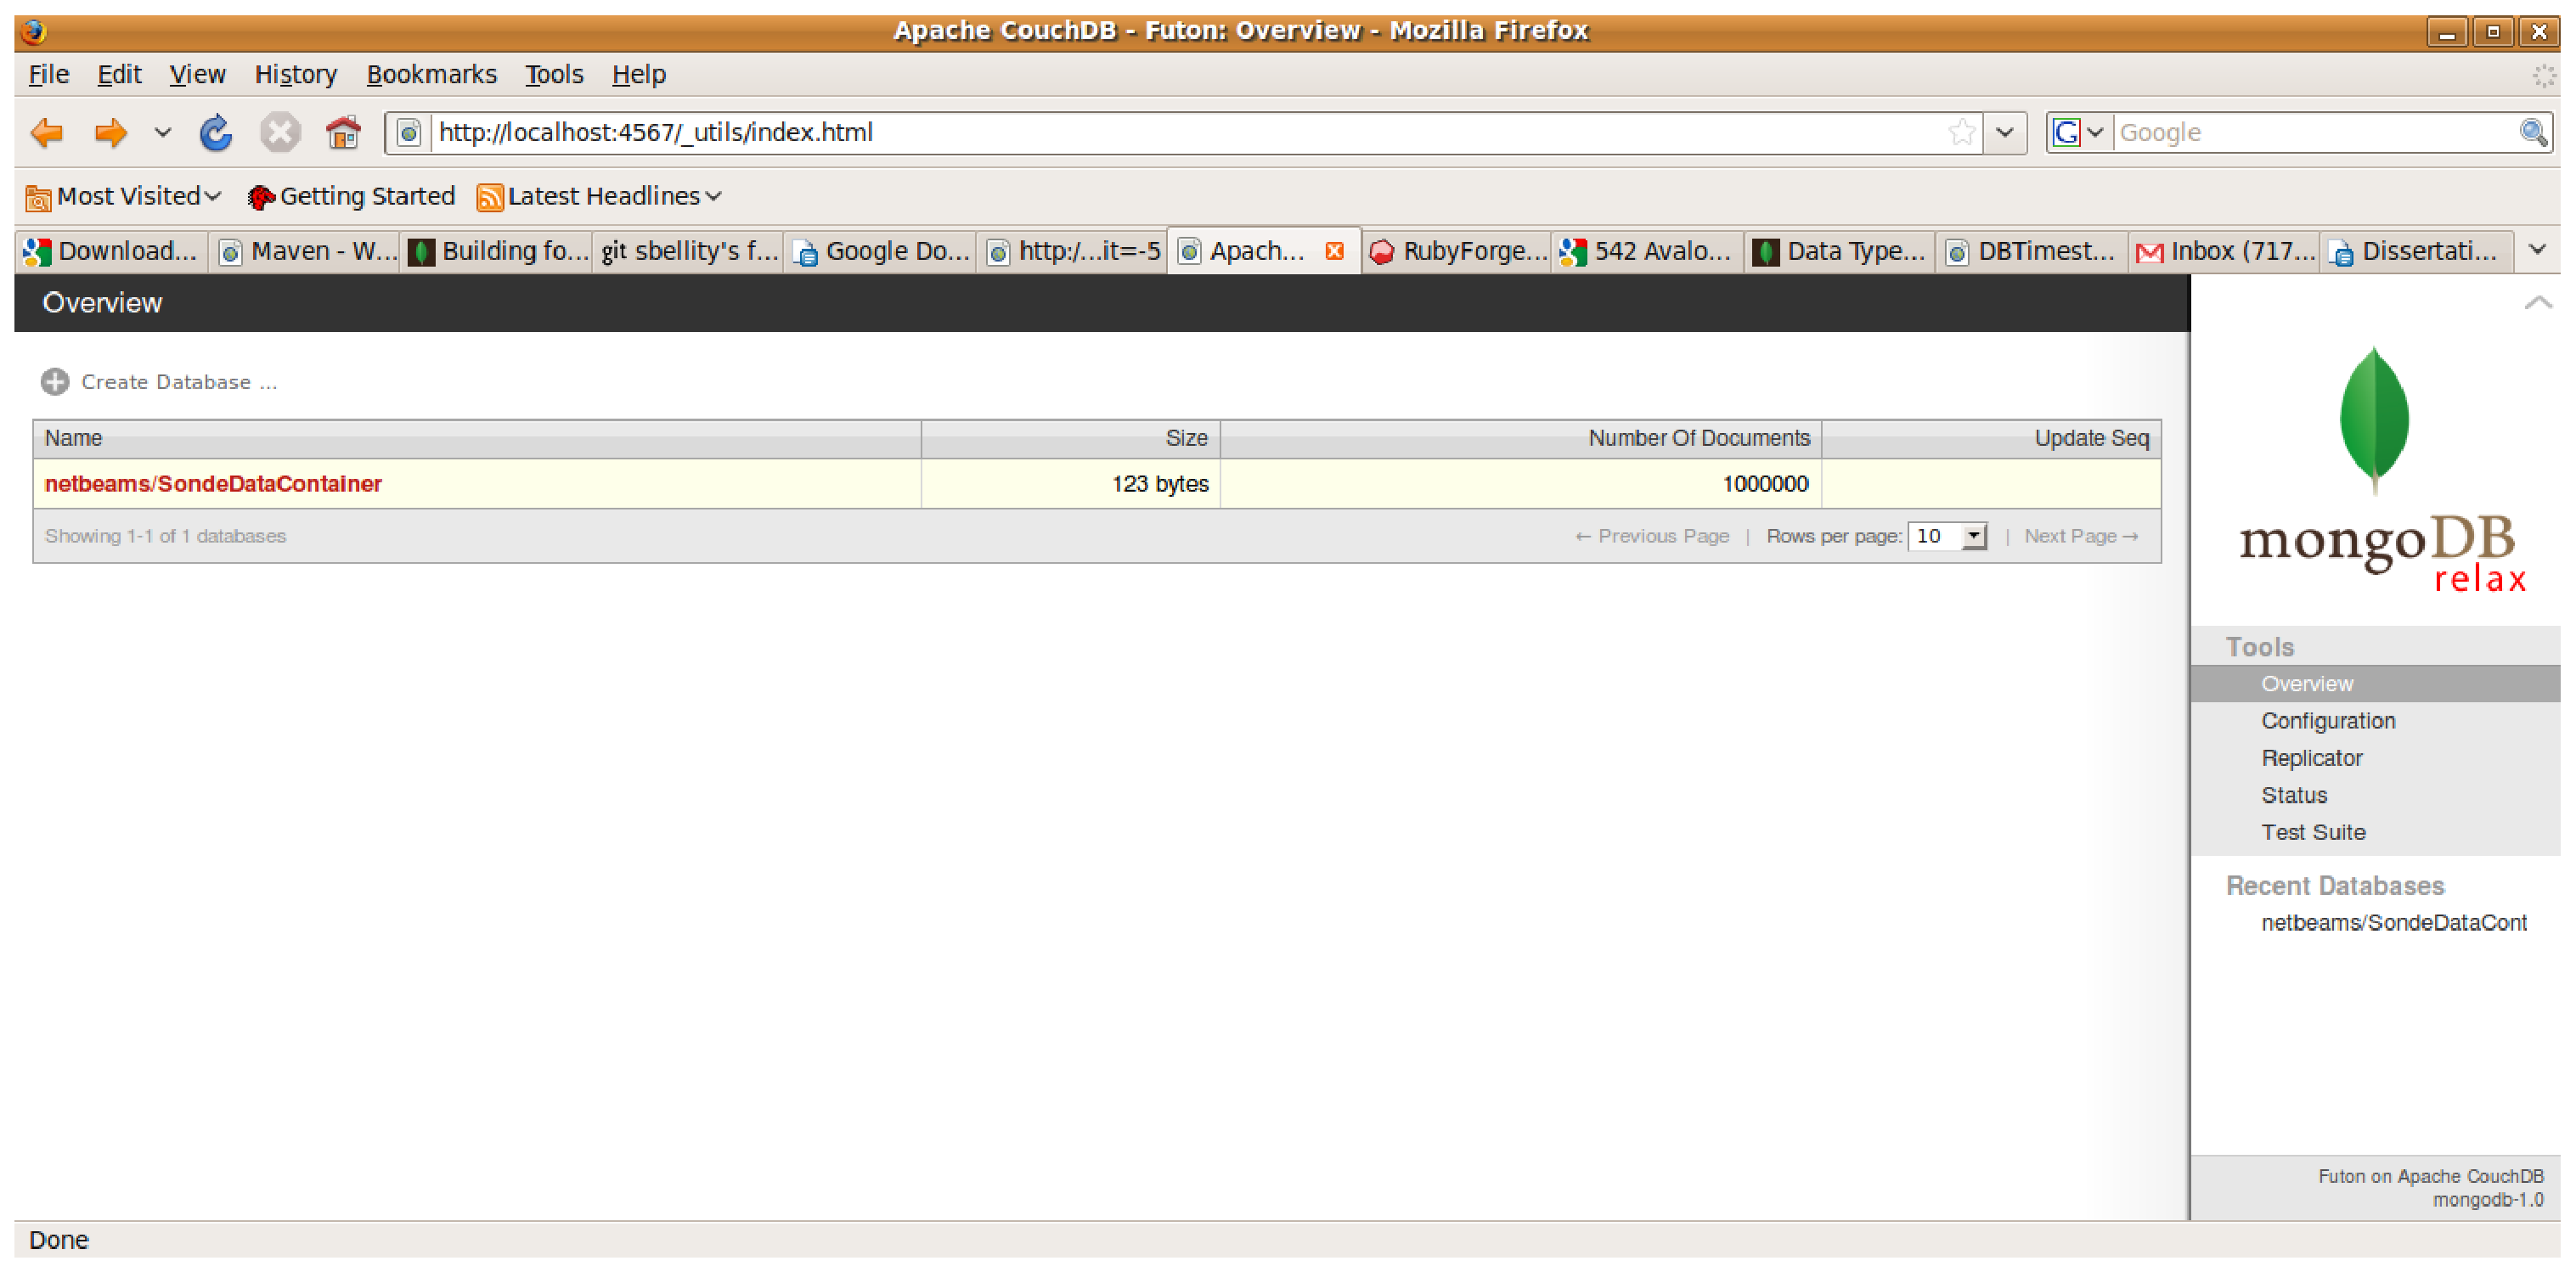
\includegraphics[scale=0.6]{../diagrams/view-collections-instance-browser-futondb}
  \caption{Viewing a partial list of data using the Futon for CouchDB/MongoDB}
  \label{fig:view-collections-instance-browser-futondb}
\end{figure}

The collection is composed by instances of documents that represents the YSI
Sonde type, being indexed by a document ID and the values being the keys
defined, as shown in Figure \ref{fig:view-collected-data-list-browser-futondb}.

\begin{figure}[!h]
  \centering
  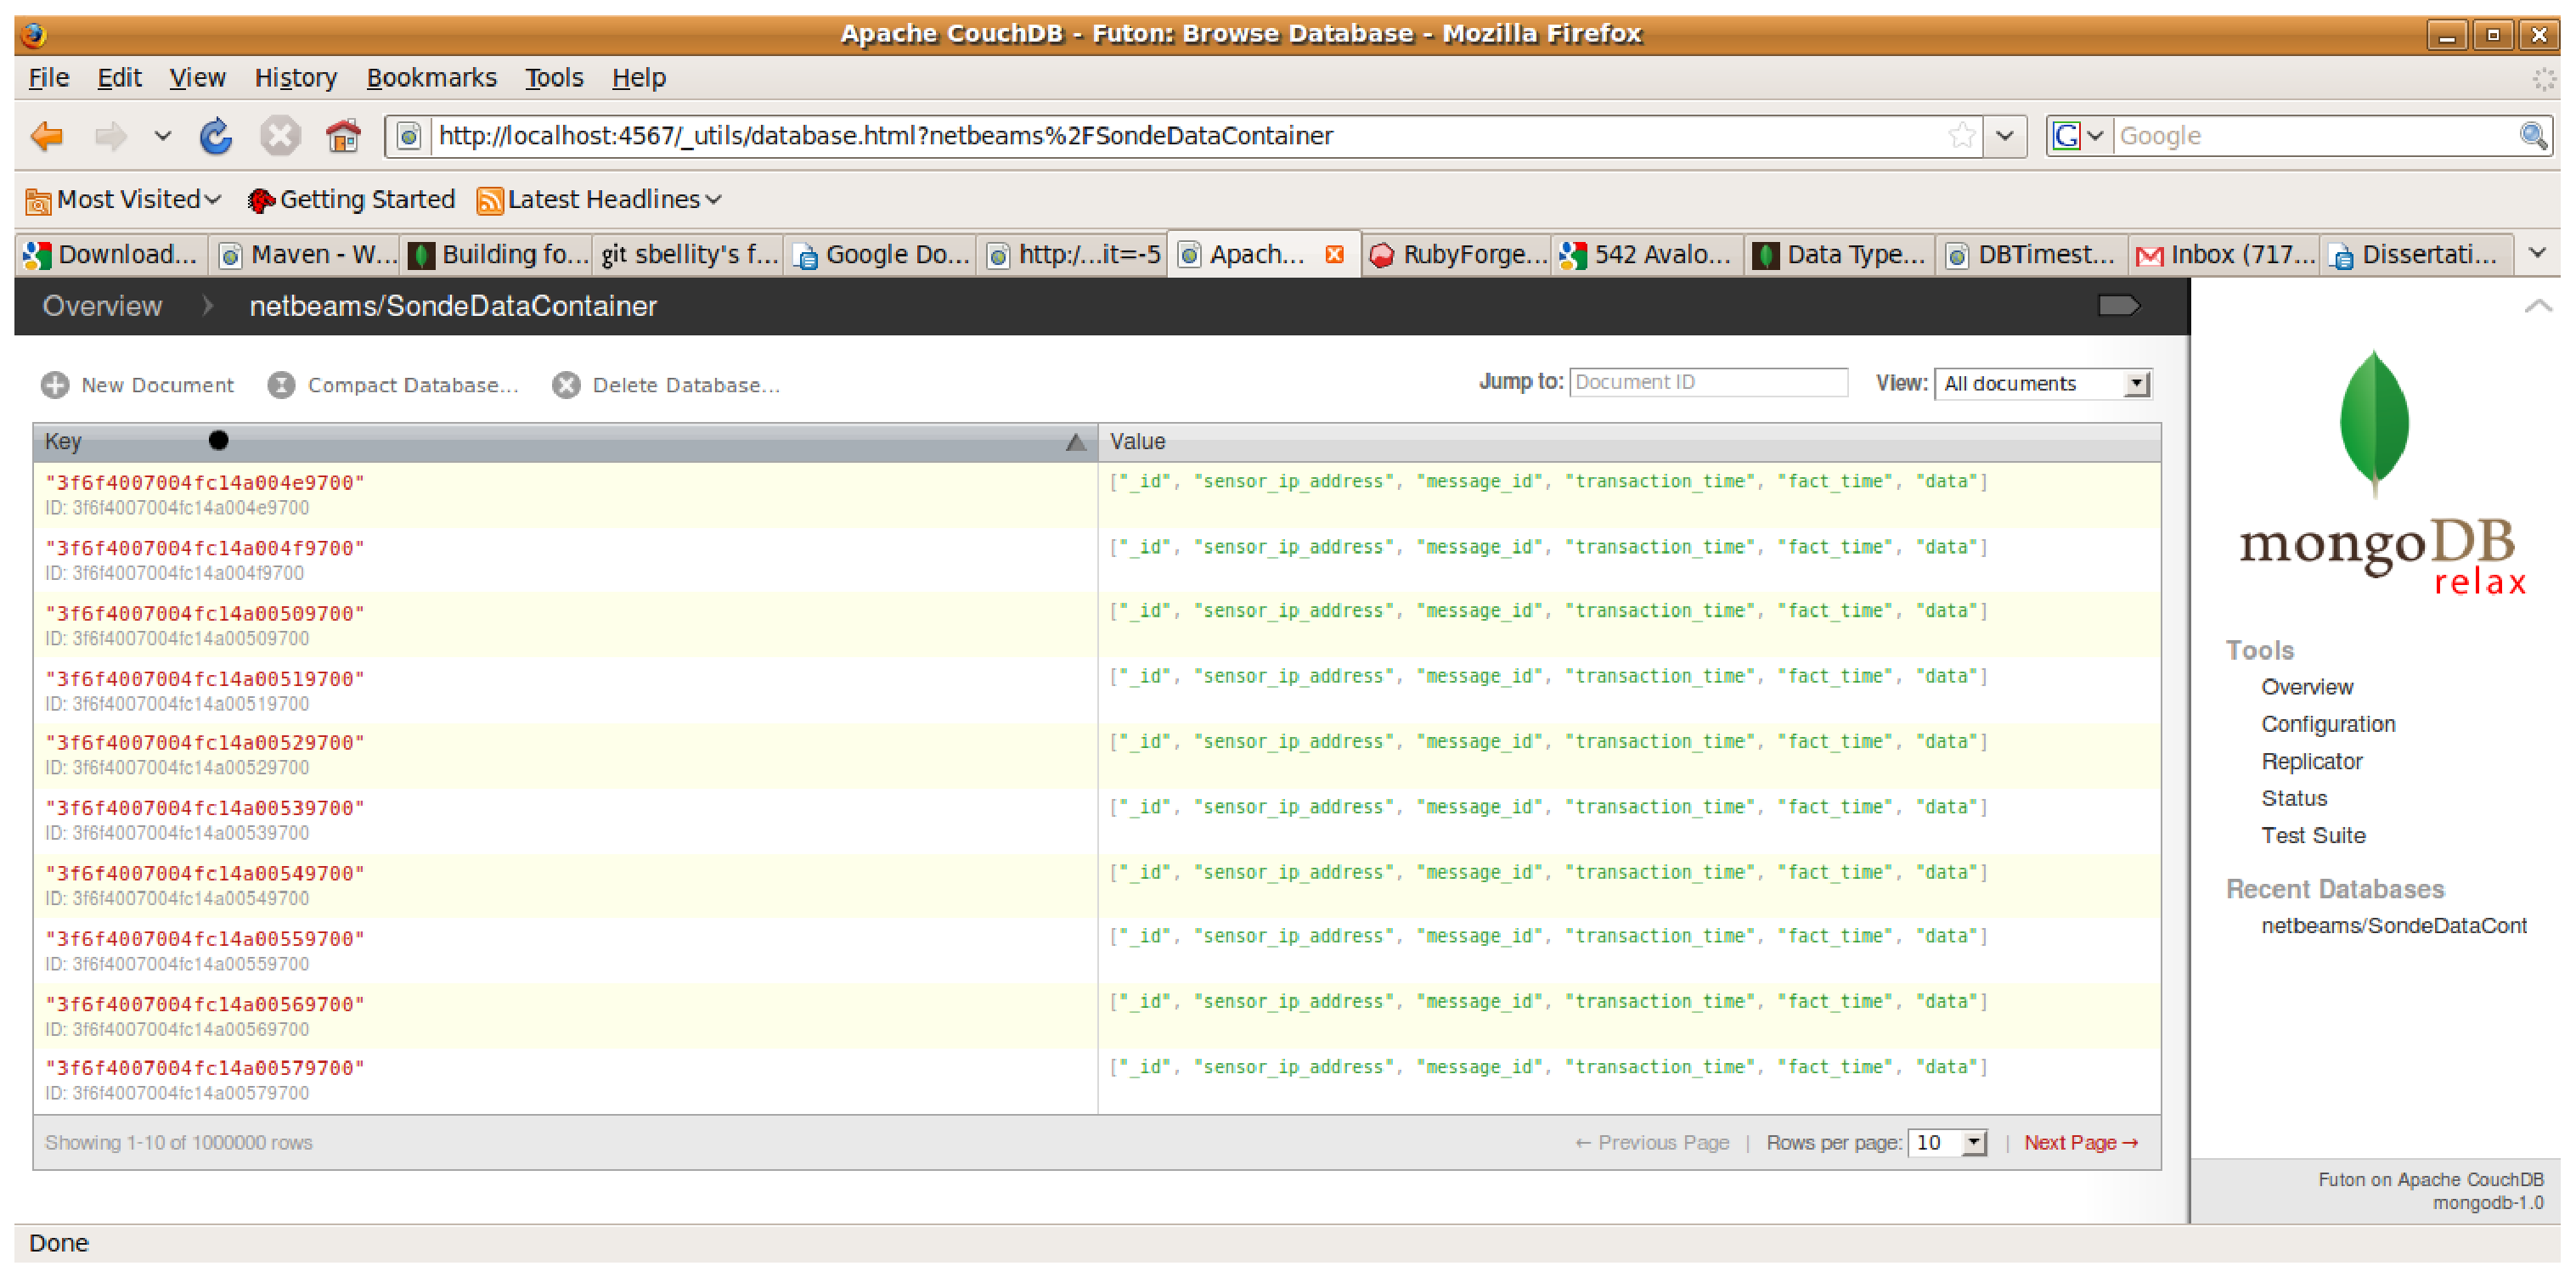
\includegraphics[scale=0.65]{../diagrams/view-collected-data-list-browser-futondb}
  \caption{Viewing a partial list of data using the Futon4CouchDB/MongoDB}
  \label{fig:view-collected-data-list-browser-futondb}
\end{figure}

By clicking in one of the items, the document properties are shown for
navigation purposes as shown in Figure
\ref{fig:view-collections-instance-browser-futondb}.

\begin{figure}[!h]
  \centering
  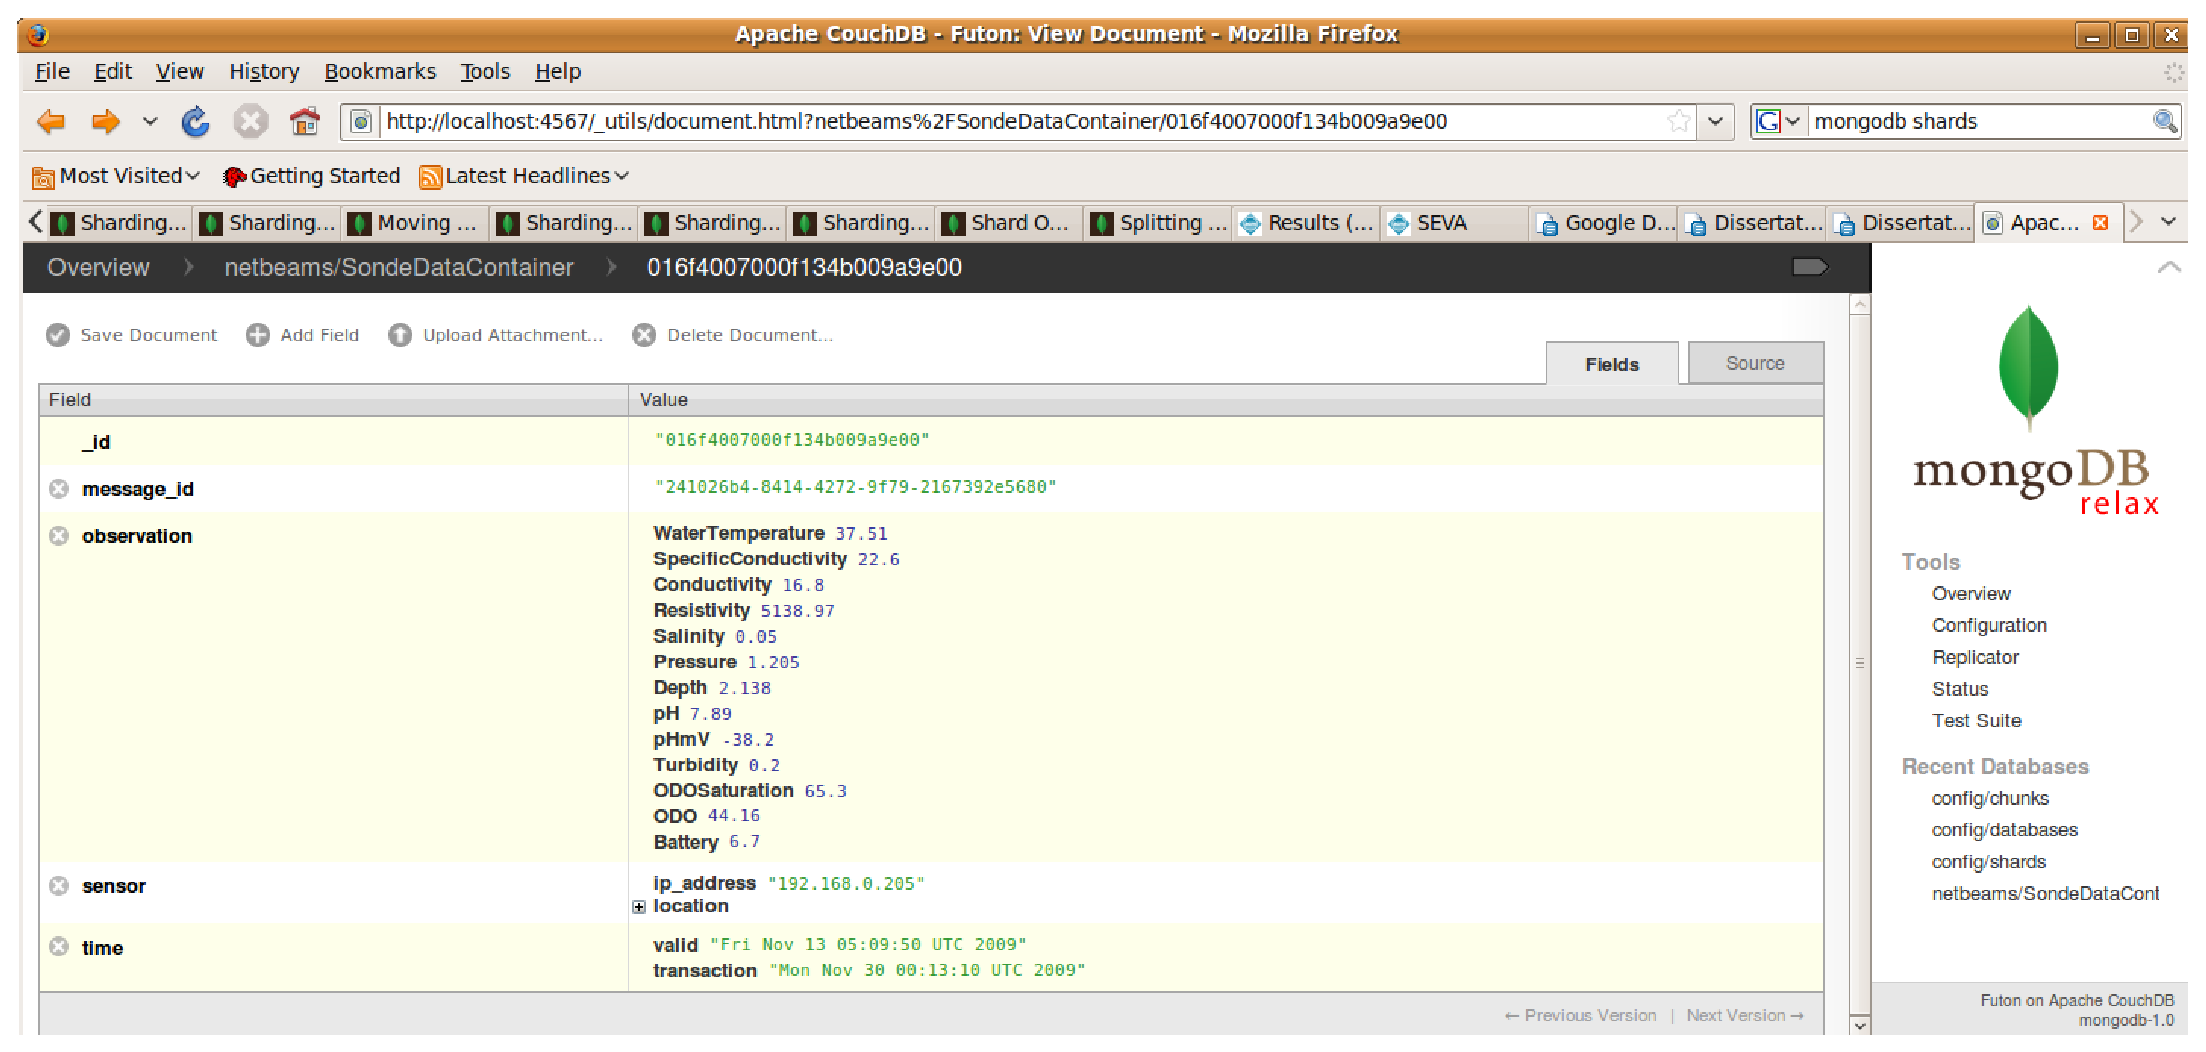
\includegraphics[scale=0.6]{../diagrams/view-collected-data-instance-browser-futondb}
  \caption{Viewing an instance of collected data using the Futon4CouchDB/MongoDB}
  \label{fig:view-collected-data-instance-browser-futondb}
\end{figure}

\subsection{Exporting Data to Spreadsheets}

mongoDB has an export facility shell called ``mongoexport''. It can export the
data in JSON format or CSV. One may also write its own export tool in any of the
languages such as Java, PHP, Python, Perl, Ruby, among others. A list of the
existing drivers in different languages is provided
athttp://www.mongodb.org/display/DOCS/Drivers. The following command can be
executed to have the exported version of the data in CSV (read the help output
of the command for details).

An example to export the data in CSV format can be seen in listing
\ref{file:mongodb-export-command}, and the resulting example containing, 1
million objects can be downloaded at
http://netbeams.googlecode.com/files/experiment-1000000-data-exported-20090913-053538.csv.tar.gz.

\subsection{Exporting Data to OPeNDAP Format}

During the experiments conducted for this work, the implementation of the
export utility to OPeNDAP was written in Python, as shown in Listing
\ref{file:experiment-export-python}. In order to execute the command, the
python programming language \cite{python} must be installed in the system. In
this way, some limited documents are exported. The following command is an
example of the execution of the export utility \ref{cmd:mongo-python-export}:

\lstset{label=cmd:mongo-python-export,caption=Query Element with specific
projection limiting the result set size}
\begin{lstlisting}
marcello@netbeams-dev:~/workspaces/netbeams/versions/v2/persistence$ python data-export-python.py 192.168.1.2:20000
\end{lstlisting}

Complete source-code listing can be reviewed in the next sections.

\section{Source-Code and Implemented Artifacts}

\lstinputlisting[language=Ant,label=file:dsp-build.xml,caption=Build
system using Apache ANT]{../../../../netbeams/versions/v2/apps/osgi-bundles/dsp/DSPDataPersistence/build.xml}

\lstinputlisting[label=file:OSGi-manifest,caption=OSGi Manifest
Descriptor]{../../../../netbeams/versions/v2/apps/osgi-bundles/dsp/DSPDataPersistence/META-INF/MANIFEST.MF}

\lstinputlisting[language=XML,label=file:dsp-config.xml,caption=DSP
Deployment
Configuration]{../../../../netbeams/versions/v2/config/deployment/config.xml}

\lstinputlisting[language=XML,label=file:dsp-matcher-config.xml,caption=DSP
Matching Rules]{../../../../netbeams/versions/v2/config/deployment/matcher_config.xml}

\lstinputlisting[language=XML,label=file:dsp-matcher-config-gumstix.xml,caption=DSP
Matching Rules
for
Gumstix]{../../../../netbeams/versions/v2/config/deployment/matcher_config-gumstix.xml}

\lstinputlisting[language=XML,label=file:dsp-data-persistence-bootstrap.xml,caption=DSP
Message used to bootstrap the DSP Data Persistence Component]
{../../../../netbeams/versions/v2/apps/xml/samples/DSPDataPersistence_001.xml}

%TODO: add bootstrap message in case it is implemented

\lstinputlisting[language=Java,label=file:dsp-activator,caption=OSGi
Activator]{../../../../netbeams/versions/v2/apps/osgi-bundles/dsp/DSPDataPersistence/src/org/netbeams/dsp/persistence/osgi/DataPersistenceActivator.java}

\lstinputlisting[language=Java,label=file:dsp-component-service,caption=OSGi
Service - Component]{../../../../netbeams/versions/v2/apps/osgi-bundles/dsp/DSPDataPersistence/src/org/netbeams/dsp/persistence/controller/DSPDataPersistence.java}

\lstinputlisting[language=Java,label=file:dsp-mongo-service,caption=DSP Data to
Mongo DB
Service]{../../../../netbeams/versions/v2/apps/osgi-bundles/dsp/DSPDataPersistence/src/org/netbeams/dsp/persistence/controller/DSPMongoCRUDService.java}

\lstset{language=XML,morecomment=[s]{!--}{--},label=stream:dsp-message-serialized-ysi,caption=DSP
Message with a YSI sonde data payload}
\begin{lstlisting}
<?xml version="1.0" encoding="UTF-8" standalone="yes"?>
<MessagesContainer uudi="24929c29-60ee-4d17-af08-64d9446277ef"
        creationTime="2009-03-06T15:17:18-0800" destinationHost="192.168.0.106">
   <MeasureMessage ContentType="org.netbeams.dsp.ysi"
         messageID="435a61f6-370f-458d-aeb7-6e92270a79cb">
      <Header>
         <CreationTime>1236381438480</CreationTime>
         
         <Producer>   
            <ComponentType>
                 org.netbeams.dsp.platform.management.component.ComponentManager
            </ComponentType>
            
            <ComponentLocator>
               <ComponentNodeId>1234</ComponentNodeId>
               <NodeAddress>192.168.0.103</NodeAddress>
            </ComponentLocator>
         </Producer>
         
         <Consumer>
            <ComponentType>
                 org.netbeams.dsp.wiretransport.client
            </ComponentType>
            
            <ComponentLocator>
               <NodeAddress>LOCAL</NodeAddress>
            </ComponentLocator>
         </Consumer>
      </Header>
      <Body>
         <SondeDataContainer>
            <soundeData date="15:17:18" time="03-06-2009">  
               <Temp>21.20</Temp>
               <SpCond>193</SpCond>
               <Cond>179</Cond>
               <Resist>5588.40</Resist>
               <Sal>0.09</Sal>
               <Press>0.084</Press>
               <Depth>0.059</Depth>
               <pH>7.98</pH>
               <phmV>-79.6</phmV>
               <ODOSat>99.5</ODOSat>
               <ODOConc>8.83</ODOConc>
               <Turbid>0.4</Turbid>
               <Battery>8.7</Battery>
            </soundeData>
         </SondeDataContainer>
      </Body>
   </MeasureMessage>
</MessagesContainer>
\end{lstlisting}

\section{Experiment Implementation}

\lstinputlisting[language=Bash,label=file:experiment-setup-executor,caption=Experiment
Main Execution Script]{../../../../netbeams/versions/v2/persistence/run-persistence-experiment}

\lstinputlisting[language=Python,label=file:experiment-setup-mongoshards,caption=Experiment
Main Execution Script]{../../../../netbeams/versions/v2/persistence/setup-mongo-shards.js}

\lstinputlisting[language=Bash,label=file:setup-os-shards-step1,caption=Experiment
Main Execution Script]{../../../../netbeams/versions/v2/persistence/setup-os-shards-step1}

\lstinputlisting[language=Bash,label=file:setup-os-shards-step2,caption=Experiment
Main Execution Script]{../../../../netbeams/versions/v2/persistence/setup-os-shards-step2}

\lstinputlisting[language=Python,label=file:experiment-export-python,caption=Data
Export to from mongoDB to OPeNDAP format.]{../../../../netbeams/versions/v2/persistence/data-export-python.py}

\lstinputlisting[language=Python,label=file:experiment-scenarios,caption=Experiment
Scenarios Implementation]{../../../../netbeams/versions/v2/persistence/experiment-client-scenarios.js}

\lstinputlisting[language=Java,label=file:main-ysi-data-handler,caption=The
DSP YSI Sonde Data Handler]{../../../../netbeams/versions/v2/apps/xml/jaxb/sonde/java-src/org/netbeams/dsp/ysi/SondeDataType.java}

\lstinputlisting[language=Java,label=file:random-ysi-data-generator,caption=Random
Test Data Generator]{../../../../netbeams/versions/v2/apps/osgi-bundles/dsp/DSPSondeProducer/src/org/netbeams/dsp/ysi/SondeTestData.java}

\lstinputlisting[language=Java,label=file:experiment-dsp-java-executor,caption=Inserting
Random Data to MongoDB]{../../../../netbeams/versions/v2/apps/osgi-bundles/dsp/DSPDataPersistence/src/org/netbeams/dsp/persistence/controller/DSPMessageToMongoDBExperiment.java}

\subsection{Experiment Execution Output}

\lstset{label=file:mongodb-ysi-data-format,caption=JSON representation of the
data produced by a YSI sensor on mongoDB}
\begin{lstlisting}
{
    "_id" : ObjectId("5d6f40078ec8074bba980900"),
    "message_id" : "020d82e1-18b2-4fe2-800c-a0f68e22ea86",
    "sensor" : {
        "ip_address" : "192.168.0.91",
        "location" : {
            "latitude" : 37.89155,
            "longitude" : -122.4464
        }
    },
    "time" : {
        "valid" : "Wed Nov 04 2009 02:30:12 GMT-0800 (PST)",
        "transaction" : "Sat Nov 21 2009 03:01:33 GMT-0800 (PST)"
    },
    "observation" : {
        "WaterTemperature" : 88.58,
        "SpecificConductivity" : 180.5,
        "Conductivity" : 167.3,
        "Resistivity" : 491.89,
        "Salinity" : 0.06,
        "Pressure" : 1.109,
        "Depth" : 2.642,
        "pH" : 7.11,
        "pHmV" : -42.9,
        "Turbidity" : 0.2,
        "ODOSaturation" : 72.4,
        "ODO" : 10.85,
        "Battery" : 2.7
    }
}
\end{lstlisting}

\lstset{label=file:rtc-ysi-opendap,caption=HTTP GET Request x Response to the OPeNDAP server at SF-BEAMS}
\begin{lstlisting}
http://sfbeams.sfsu.edu:8080/opendap/sfbeams/data_ctd/rtc_ctd5-ysimoor/real-time/sfb_CTD5_PUF.dat.ascii?
GET /opendap/sfbeams/data_ctd/rtc_ctd5-ysimoor/real-time/sfb_CTD5_PUF.dat.dods?&Month=11&Day=12 HTTP/1.1

HTTP/1.x 200 OK
Server: Apache-Coyote/1.1
Last-Modified: Thu, 12 Nov 2009 17:55:06 GMT
XDODS-Server: Server-Version-Unknown
XOPeNDAP-Server: bes/3.5.1 freeform_handler/3.7.5, netcdf_handler/3.7.6
XDAP: 3.2
Content-Description: dods_data
Content-Type: text/txt
Date: Sun, 15 Nov 2009 03:08:45 GMT

Dataset: sfb_CTD5_PUF.dat
YSI_REALTIME_CSV.Month, YSI_REALTIME_CSV.Day, YSI_REALTIME_CSV.Year, YSI_REALTIME_CSV.Hour, YSI_REALTIME_CSV.Min, YSI_REALTIME_CSV.Sec, YSI_REALTIME_CSV.WaterTemperature, YSI_REALTIME_CSV.SpecificConductivity, YSI_REALTIME_CSV.Conductivity, YSI_REALTIME_CSV.Resistivity, YSI_REALTIME_CSV.TDS, YSI_REALTIME_CSV.Salinity, YSI_REALTIME_CSV.Pressure, YSI_REALTIME_CSV.Depth, YSI_REALTIME_CSV.pH, YSI_REALTIME_CSV.pHmV, YSI_REALTIME_CSV.Turbidity, YSI_REALTIME_CSV.ODOSaturation, YSI_REALTIME_CSV.ODO, YSI_REALTIME_CSV.Chlor, YSI_REALTIME_CSV.Chlor_RFU, YSI_REALTIME_CSV.Battery, YSI_REALTIME_CSV.InstSN
11, 12, 2009, 16, 30, 51, 13.78, 4.3945, 3.4532, 0, 28.56, 28.35, 2.65, 2.651, 7.9, -54.7, 9, -99999, -99999, 3.7, 1, 9.4, -99999
11, 12, 2009, 16, 36, 50, 13.78, 4.4095, 3.4642, 0, 28.66, 28.46, 2.628, 2.63, 7.91, -54.9, 11.9, -99999, -99999, 4, 1.1, 9.4, -99999
11, 12, 2009, 16, 42, 51, 13.77, 4.3943, 3.4515, 0, 28.56, 28.35, 2.631, 2.632, 7.9, -54.9, 9.8, -99999, -99999, 3.6, 1, 9.4, -99999
11, 12, 2009, 16, 48, 50, 13.76, 4.3893, 3.447, 0, 28.53, 28.32, 2.628, 2.63, 7.9, -54.8, 10.6, -99999, -99999, 3.8, 1, 9.4, -99999
\end{lstlisting}

\lstset{label=file:mongodb-export-command,caption=Export Command to CSV format}
\begin{lstlisting}
mongoexport -d netbeams -c SondeDataContainer --dbpath data --csv -f "_id,sensor_ip_address,transaction_time,fact_time,data.temperature,data.sp_condition,data.condition,data.resistence,data.salinitude,data.pressure,data.depth,data.ph,data.pH_mv,data.odo_sat,data.odo_condition,data.turbidity,data.battery" -o logs/experiment-483840-data-exported-20091129-190207.csv

Sun Nov 29 19:07:04 query netbeams.SondeDataContainer ntoreturn:0 reslen:2258 nscanned:101 { query: {}, $snapshot: 1 }  nreturned:101 202ms
Sun Nov 29 19:07:04 getmore netbeams.SondeDataContainer cid:7749363894863150628 ntoreturn:0 query: { query: {}, $snapshot: 1 }  bytes:1048562 nreturned:47661 1767ms
...
...
Sun Nov 29 19:10:18 getmore netbeams.SondeDataContainer cid:7749363894863150628 ntoreturn:0 query: { query: {}, $snapshot: 1 }  bytes:793098 nreturned:36049 1975ms
exported 2419200 records
\end{lstlisting}

\lstinputlisting[label=file:experiment-export-python-results,caption=Data
Export to from mongoDB to OPeNDAP format.]{../../../../netbeams/versions/v2/persistence/export-mongodb-to-sfbeams.csv}